\documentclass[]{article}
\usepackage[a4paper]{geometry}
\usepackage{graphicx}
\usepackage{titling}
\usepackage{listings}
\begin{document}

\title{Project Datacommunicatie}
\author{Enver Bral \\ Fr\'ed\'erique De Baerdemaeker \\ Ruben Taelman \\ Felix Van der Jeugt}
\date{Academiejaar 2012 - 2013}
\maketitle

\begin{section}*{Broncodering}

    \begin{subsection}*{Vraag 1}

        We verkrijgen volgende output bij het uitvoeren van
        \texttt{FrequencyCounter.m}:

        \begin{lstlisting}
            0.5443    0.0024    0.0031    0.0040
            0.0019    0.0045    0.0001    0.0026
            0.0020    0.0001    0.0044    0.0029
            0.0045    0.0025    0.0018    0.4189
        \end{lstlisting}

        Dit zijn de relatieve frequenties voor elk macroblok. De
        macroblokken zijn hier als volgt genummerd: We zetten de rijen
        van het macroblok na elkaar, en lezen als een binair getal.

        Zo wordt het macroblock \texttt{[1 0;0 1]} omgezet naar
        \texttt{1 0 0 1} en krijgt het nummer $9$.

        Handmatige huffman:

        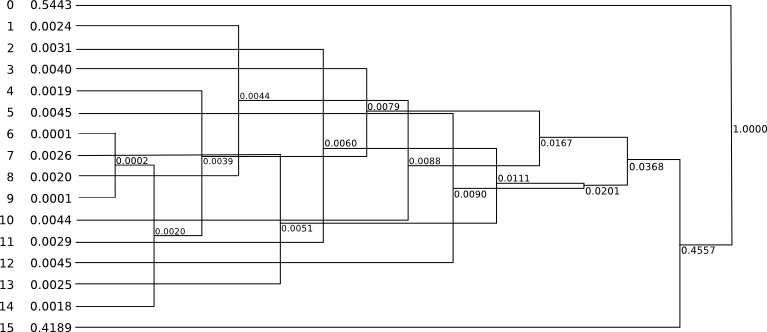
\includegraphics[width=\textwidth]{manual_huffman.png}

    \end{subsection}
    
        \begin{subsection}*{Vraag 3}

        We verkrijgen volgende grafiek bij het uitvoeren van
        \texttt{FrequencyCounter.m}:

        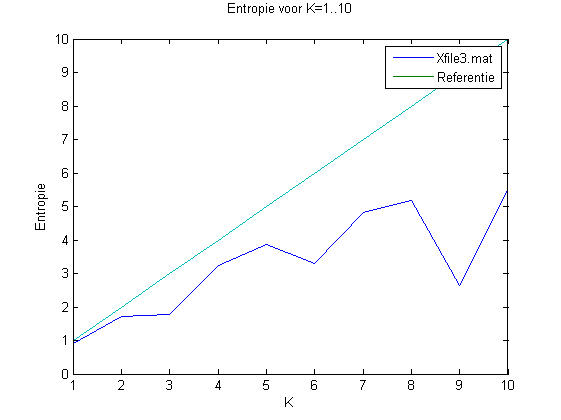
\includegraphics{vraag1_3.png}
		Hierop kunnen we de entropie zien van de macrosymbolen van grootte K. De referentielijn is hier een rechte, dit is logisch aangezien de entropie maximaal is wanneer alle symbolen met gelijke kans voorkomen.
		Vanaf K=8 komen er symbolen voor die met frequentie 0 voorkomen, dus hier is de log2 -oneindig, dus de entropie wordt hier ook oneindig groot.

    \end{subsection}
\end{section}
\begin{section}*{Kanaalcodering}
\end{section}
\begin{section}*{Volledig systeem}
\end{section}
\end{document}
